\documentclass[]{exam}
\usepackage{amssymb}
\usepackage{amsfonts}
\usepackage{amsmath}
\usepackage{amsthm}
\usepackage[top=1in, bottom=1.5in, left=1in, right=1in]{geometry}
\usepackage{tikz}
\usepackage{pgfplots}
\usepackage{empheq}
\usepackage{mathrsfs}
\checkboxchar{$\Box$}
\usepackage{graphicx}
\usepackage{caption}
\usepackage{float}
\usepackage{enumerate}
\usepackage{comment}
\usepackage{multicol}
\usepackage{color}
\usepackage{advdate}
\usepackage{gensymb}
\usetikzlibrary{arrows}
\usepackage{multirow}
\usepackage{arydshln}
\usepackage{verbatim}
\usepackage{systeme}


\usepackage{pgfkeys,pgfcalendar}

\newcount\pgfdatecount
\newcommand{\tomorrow}{%
\pgfcalendardatetojulian{\year-\month-\day+1}{\pgfdatecount}
\pgfcalendarjuliantodate{\the\pgfdatecount}{\myyear}{\mymonth}{\myday}
\pgfcalendarmonthname{\mymonth}\space\myday,\space\myyear%
}

\newcommand{\advanceday}[1][1]{
\begingroup
\AdvanceDate[#1]
\today
\endgroup}

\newcommand{\vertex}{\node[vertex]}
\tikzstyle{vertex}=[circle, draw, inner sep=0pt, minimum size=6pt]
\usepackage{lastpage} 
\usepackage{extramarks}
\usepackage{graphicx} 
\usepackage{tikz}
\usepackage{sectsty} 
\usepackage{amsmath,amsfonts,amsthm} 
\usepackage{wrapfig, blindtext}

% Margins
\topmargin=-0.45in
\evensidemargin=0in
\oddsidemargin=0in
\textwidth=6.5in
\textheight=9.0in
\headsep=0.25in 
\numberwithin{equation}{section}
\linespread{1.1} 
\setlength\parindent{0pt} 
\setlength\answerskip{-.075in}
\setlength\answerlinelength{.5in}
\newcommand{\myitem}{\item[-]}

% HEADER AND FOOTER
\pagestyle{headandfoot}
\runningheadrule
\runningfootrule
\firstpageheader{Kutztown University}{  }{MATH 210}
\firstpageheadrule
\runningheader{P2.H1-2}{ }{MATH 210}
\firstpagefooter{}{}{} 
\runningfooter{}{}{Page \thepage\ of \numpages}


% TITLE PAGE
\newcommand{\assignmentname}{Phase 2 -- Homework} % Assignment title
\newcommand{\coursetitle}{MATH 210 -- Mathematical Computing and Typesetting}
\newcommand{\duedate}{Due: Friday, March 6 by 11:59 PM on D2L} % Class/lecture time
\newcommand{\readsections}{\, } % Teacher/lecturer
\newcommand{\semester}{\, }
\title{
\vspace{2in}
\textmd{\textbf{\course:\ \assignmentname}}\\
\normalsize\vspace{0.1in}{\duedate}\\
\vspace{0.1in}\large{\textit{\instructor}}
\vspace{3in}
}
\author{\textbf{Author: \authorname}}
\date{Last Updated: \today}

\pointsinrightmargin
\bracketedpoints



\begin{document}
%%%%%%%%%%%%%%%%%%%%%%%%%%%%%%%%%%%%%%%%%%%%%%%%%%%%%
% COMPILE TITLES AND SUCH
%%%%%%%%%%%%%%%%%%%%%%%%%%%%%%%%%%%%%%%%%%%%%%%%%%%%%
\hspace{1in}\\ \vspace{.15in}


\begin{center}
\normalsize
 \fbox{\fbox{\parbox{5.5in}{
        {\bf Instructions:}  Upload the \texttt{tex} file for this document to your Overleaf project.  All solutions shall be completed on this packet by typing your solution in \LaTeX\, in the space provided.  All solutions should be detailed and should clearly demonstrate the process by which you arrived at the answer.  Submit the compiled \texttt{pdf} file to D2L by 11:59 PM on the due date below.  Submit only a single pdf file of your entire packet.  The question will also ask you to make calculations in Python.  Upload any Python files to the appropriate folder in your GitHub repository.  In this folder, a \texttt{py} file is to be submitted for each problem such that when the \texttt{py} file is executed, the output (as presented in Python) is the solution to the problem. Academic dishonesty will not be tolerated.  }}}
\end{center}

\vspace{.5cm}

\begin{center}
	\Huge\textsc{
	\assignmentname}\\[4pt]
        \Large{\textsc{\coursetitle}\\[10pt]}
        \Large{\textsc{\duedate}\\[8pt]}
        \Large{\textsc{\readsections}\\[8pt]}
\end{center}

\vspace{1cm}

%%%%%%%%%%%%%%%%%%%%%%%%%%%%%%%%%%%%%%
% Uncomment the syntax below when you type up the solutions and type 
% your name.
\begin{center}
	\large{\textsc{\textcolor{red}{Solutions by Brooks Emerick}}}
\end{center}
\vfill

%%%%%%%%%%%%%%%%%%%%%%%%%%%%%%%%%%%%%%
% Reminders:
%%%%%%%%%%%%%%%%%%%%%%%%%%%%%%%%%%%%%%
Remember to begin your \texttt{py} file with \texttt{import numpy as np} and \verb|import matplotlib.pyplot as plt|.  For some of the problems below, use \texttt{import scipy.linalg as la}.


% Blank Page
\clearpage

\begin{questions}
%%%%%%%%%%%%%%%%%%%%%%%%%%%%%%%%%%%%%%
% NUMBER 1 
%%%%%%%%%%%%%%%%%%%%%%%%%%%%%%%%%%%%%%
\question Create a Python program that will solve the following system of equations by setting up the proper matrix equation and solving it in two ways: one way using $\texttt{la.inv}$ and another using $\texttt{la.solve}$:

\begin{center}
	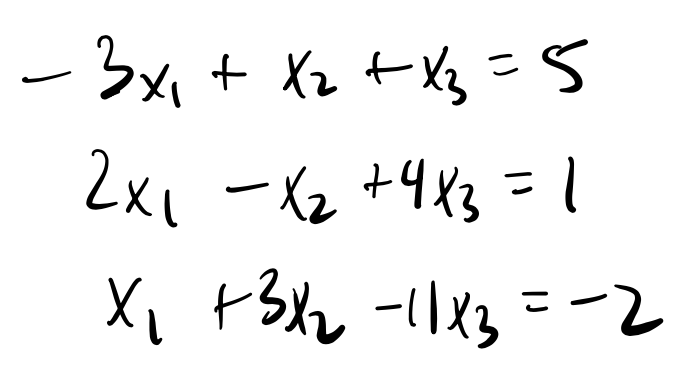
\includegraphics[width = .35\textwidth]{P2_HW_Figure_1.png}
\end{center}

Your final output in Python should print the solution vector $\boldsymbol{x}$.  Type up the handwritten system above, by replacing the picture with the actual typed up equations in \LaTeX.  You will have to use the \texttt{align} environment and align the equations at the equal sign. In the space below, type the matrix $A$, the vector $\boldsymbol{x}$, and the vector $\boldsymbol{b}$.\\

\textsc{Solution:} \\

The system above can be typed up as below:
\begin{align*}
	-3x_1  +  x_2  + x_3  &=  5 \\ 
	2x_1  -  x_2  +  4x_3  &= 1 \\ 
	x_1  +  3x_2  -  11x_3  &= -2 \end{align*}
  
This set of linear equations can be represented by the matrix equation $A\boldsymbol{x} = \boldsymbol{b}$, where 
\[ A = \begin{bmatrix} 
	-3 & 1 & 1 \\ 
	2 & -1 & 4 \\ 
	1 & 3 & -11 \end{bmatrix}, \qquad \boldsymbol{x} = \begin{bmatrix}
		x_1 \\ x_2 \\ x_3 \end{bmatrix}, \qquad \text{and} \quad 
		\boldsymbol{b} = \begin{bmatrix} 5 \\ 1 \\ -2 \end{bmatrix}.\]
\pagebreak


%%%%%%%%%%%%%%%%%%%%%%%%%%%%%%%%%%%%%%
% NUMBER 2
%%%%%%%%%%%%%%%%%%%%%%%%%%%%%%%%%%%%%%
\question Create a \texttt{py} file in Python that defines the following matrices.  I want you to explore the built-in functions that are used to create large matrices.  Each of these matrices below can be constructed in one or two lines \textit{without} a for loop. 

\begin{enumerate}
\item[$a.)$] Define $A$ as a $30\times 20$ matrix of threes using \texttt{np.ones}.
\item[$b.)$] Using \texttt{np.reshape} and \texttt{np.arange}, define $B$ as the $10 \times 10$ matrix:
\[\displaystyle \begin{bmatrix} 1 & 11 & \cdots & 91 \\ 2 & 12 & \cdots & 92 \\ 
\vdots & \vdots & \ddots & \vdots \\
10 & 20 & \cdots & 100\end{bmatrix}.\]
\item[$c.)$] Using \texttt{np.diag} and \texttt{np.ones} more than once, define $C$ as the $16\times 16$ matrix: 
\[\displaystyle \begin{bmatrix} -2 & 1 & 0 & 0 &  \cdots & 0 & 1 \\ 
1 & -2 & 1 & 0 & \cdots & 0 & 0 \\ 
0 & 1 & -2 & 1  & \cdots & 0 & 0 \\ 
\vdots & \ddots &  \ddots & \ddots &  \ddots & \ddots & \vdots \\
0 & 0  & \cdots & 1& -2 & 1 & 0\\
0 & 0  & \cdots & 0&  1& -2 & 1\\
1 & 0  & \cdots & 0 & 0  &1& -2 \end{bmatrix}.\]
(This is a \textit{differentiation matrix}.) Use the command \texttt{plt.spy(C)} to plot the sparsity of this matrix in Figure 1. 

\item[$d.)$] Read about \texttt{la.toeplitz} and use it to make the matrix from part $c.)$.  Call this matrix $D$.

\item[$e.)$] Use \texttt{la.toeplitz}, \texttt{np.triu}, and whatever else to make the following $8\times 8$ matrix:
\[\displaystyle E = \begin{bmatrix} 1 & 2 & 3 & \cdots & 8  \\ 
0  & 1 & 2 & \cdots & 7 \\ 
\vdots & \ddots & \ddots & \ddots & \vdots \\
0 &  \cdots & 0 & 1 & 2 \\
0 &  \cdots & 0 & 0 & 1\end{bmatrix}.\]
Use the command \texttt{plt.spy(E)} to plot the sparsity of this matrix in Figure 2.
 
\item[$f.)$] Use \texttt{la.toeplitz} and whatever else to create the following $8\times 8$ matrix:
\[\displaystyle F = \begin{bmatrix} 1 & \frac{1}{2} & \frac{1}{3} & \cdots & \frac{1}{8}  \\ 
\frac{1}{2}  & 1 & \frac{1}{2} & \cdots & \frac{1}{7} \\ 
\vdots & \ddots & \ddots & \ddots & \vdots \\
\frac{1}{7} &  \cdots & \frac{1}{2} & 1 & \frac{1}{2} \\
\frac{1}{8} &  \cdots & \frac{1}{3} & \frac{1}{2} & 1\end{bmatrix}.\]

\end{enumerate}

\pagebreak

%%%%%%%%%%%%%%%%%%%%%%%%%%%%%%%%%%%%%%
% NUMBER 3
%%%%%%%%%%%%%%%%%%%%%%%%%%%%%%%%%%%%%%
\question In this problem you are trying to find an approximation to the periodic function $f(x) = e^{\sin(x-1)}$ over one period, $0\leq x \leq 2\pi$.  In Python, let \verb|x = np.linspace(0, 2*np.pi, int(200))| and \texttt{y} be the evaluation of $f$ at those points.
\begin{enumerate}
	\item[$a.)$] Fit a degree 7 polynomial to these data by using the normal equations and the appropriate truncated Vandermonde matrix $A$. 
	\item[$b.)$] Fit the following sinusoidal function 
		\[ f(x) = c_0 + c_1 \cos(x) + c_2 \sin(x) + c_3\cos(2x) + c_4\sin(2x) \]
		using \verb|scipy.optimize.curve_fit|.  
	\item[$c.)$] Plot the original function, and the two approximations together on a well-labeled graph. In your \LaTeX\, report, include the graph below. 
	
	\begin{center}
		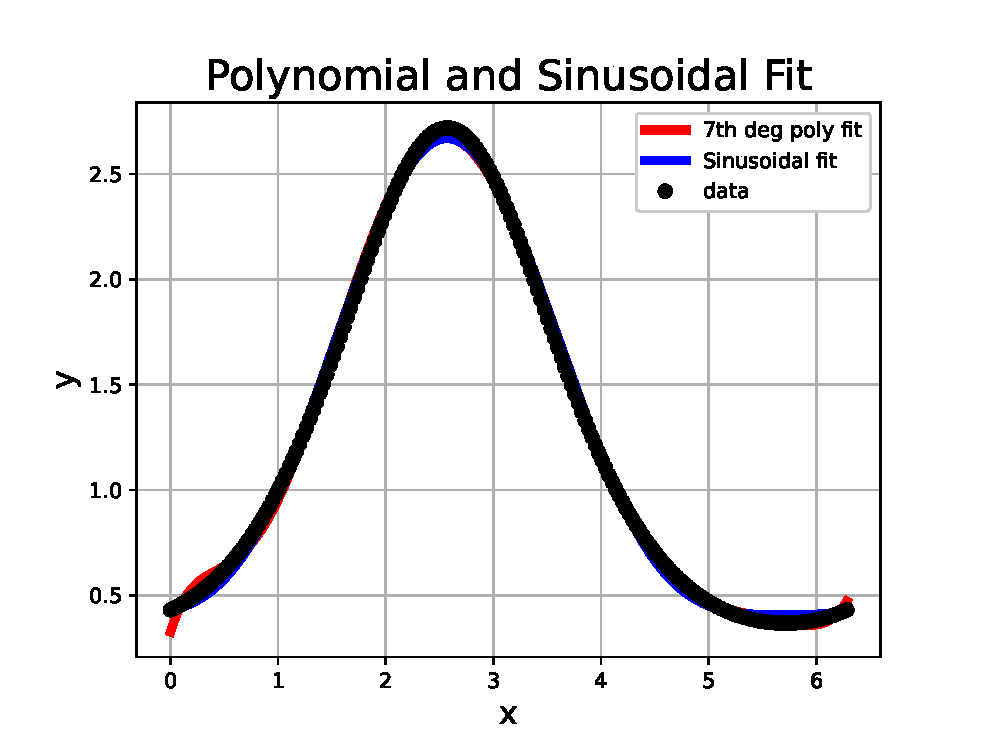
\includegraphics[width = .7\textwidth]{P2_HW_Figure_2.eps}
	\end{center}
	\item[$d.)$] Compute the $R^2$ value for each function and print the value for each model.
\end{enumerate}




\end{questions}
\end{document} 
